% !TeX root = ba.tex

\section{Experiments}

\subsection{Datasets and Network Architectures}



\subsection{Results}
 
 We trained models on each of the following benchmark data sets:

\begin{itemize}
	\item MNIST: $28\times28$ grayscale images of handwritten digits (60,000  images for training / 10,000  images for testing) \cite{mnist}
	\item Fashion-MNIST:  $28\times28$ grayscale images of fashion items (60,000 images for training / images 10,000 for testing) \cite{fashion}
	\item SVHN: $32\times32$ color images of house numbers (73,257  images for training / 26,032 images for testing) \cite{svhn}
	\item CIFAR-10: $32\times32$ color images (50.000  images for training / 10.000  images for testing) \cite{cifar}
\end{itemize}

Each of the four data sets consist of ten classes.

As baseline architectures we trained convolutional networks utilizing max-pooling,
batch-normalization \citep{batchnorm} and dropout \citep{dropout}.
Training capsule networks can be comparatively more difficult in practice, therefore we had to carefully construct well-suited architectures:

For the MNIST data set we used three layer CapsNet like that of \citet{capsules}, but with only 64 convolutional kernels in the first layer. \\
For the Fashion-MNIST and the SVHN data sets we used CapsNets with two convolutional layers in the beginning, followed by the primary capsule layer and the class capsules. \\
Simple CapsNets however don't perform very well on more complex data like CIFAR-10 \citep{complex}, therefore we use a modified DCNet \citep{denseanddiverse} with three convolutional capsule layers and a non-of-the-above category for the dynamic routing. \\
We train all CapsNets using margin loss and the reconstruction loss for regularization \citep{capsules}, and we use three iterations in the dynamic routing. \\
All CapsNets as well as ConvNets are trained with the Adam optimizer \citep{adam}. \\
For more details on the model architectures, please refer to the following tables: \todo{architecture tables}

\begin{table}
	
	\caption{CapsNet on SVHN}
	\begin{tabular}{|c|c|}
		\hline 
	Layer	& Output Shape \\ 
		\hline 
	Conv $64$ $5\times5$, valid, ReLU, BN	&  $28\times28\times64$ \\ 
		\hline 
	Conv $256$ $5\times5$, valid, Leaky ReLU, BN	&  $24\times24\times256$\\ 
		\hline 
	Primary Conv Caps, $64$ $9\times9$, dim=$8$	stride=$2$ &  $8\times8\times64\times8$\\ 
		\hline 
	Class Caps, dim=$16$	&  $10\times16$\\ 
		\hline
		& \\
		\hline
	FC 2048, ReLU	& 2048 \\
		\hline
	FC 4096, ReLU	& 4096 \\
		\hline
	FC 3072, sigmoid	& 3072\\
		\hline
	\end{tabular}

	\caption{ConvNet on SVHN}
	\begin{tabular}{|c|c|}
		\hline 
	Layer	&  Output Shape \\ 
		\hline 
	Conv $32$ $5\times5$, same,	ReLU & $32\times32\times32$ \\ 
		\hline 
	Max-Pooling $2\times2$, Dropout 0.15, BN	&  $16\times16\times32$ \\ 
		\hline 
	Conv $64$ $3\times3$, same, ReLU	& $16\times16\times64$ \\ 
		\hline 
	Max-Pooling $2\times2$, Dropout 0.15, BN	& $8\times8\times64$ \\
		\hline
	Conv $128$ $3\times3$, same, ReLU	& $8\times8\times128$ \\
		\hline
	Dropout 0.15, BN	& $8\times8\times128$ \\
		\hline
	FC 1024, ReLU, Dropout 0.5 & 1024 \\
		\hline
	FC 10 & 10\\
		\hline
	\end{tabular}

\end{table}

\begin{table}

	\caption{CapsNet on Fashion-MNIST}
	\begin{tabular}{|c|c|}
		\hline 
		Layer	& Output Shape \\ 
		\hline 
		Conv $32$ $3\times3$, valid, ReLU, BN	&  $26\times26\times32$ \\ 
		\hline 
		Conv $32$ $3\times3$, valid, Leaky ReLU, BN	&  $24\times24\times32$\\ 
		\hline 
		Primary Conv Caps, $16$ $9\times9$, dim=$8$	stride=$2$ &  $8\times8\times16\times8$\\ 
		\hline 
		Class Caps, dim=$16$	&  $10\times16$\\ 
		\hline 
		& \\
		\hline
		FC 512, ReLU	& 512 \\
		\hline
		FC 1024, ReLU	& 1024 \\
		\hline
		FC 784, sigmoid	& 784 \\
		\hline
	\end{tabular}

	\caption{ConvNet on Fashion-MNIST}
	\begin{tabular}{|c|c|}
		\hline 
		Layer	&  Output Shape \\ 
		\hline 
		Conv $32$ $5\times5$, same,	ReLU & $28\times28\times32$ \\ 
		\hline 
		Max-Pooling $2\times2$, Dropout 0.15, BN	&  $14\times14\times32$ \\ 
		\hline 
		Conv $64$ $3\times3$, same, ReLU	& $14\times14\times64$ \\ 
		\hline 
		Max-Pooling $2\times2$, Dropout 0.15, BN	& $7\times7\times64$ \\
		\hline
		Conv $128$ $3\times3$, same, ReLU	& $7\times7\times128$ \\
		\hline
		Dropout 0.15, BN	& $7\times7\times128$ \\
		\hline
		FC 1024, ReLU, Dropout 0.5 & 1024 \\
		\hline
		FC 10 & 10\\
		\hline
	\end{tabular} 

\end{table}

\begin{table}

	\caption{CapsNet on MNIST}
	\begin{tabular}{|c|c|}
		\hline 
		Layer	&  Output Shape \\ 
		\hline 
		Conv $64$ $9\times9$, valid, ReLU, BN & $24\times24\times64$ \\ 
		\hline 
		Primary Conv Caps, $32$ $9\times9$, dim=$8$, stride=2	&  $8\times8\times32\times8$ \\ 
		\hline 
		Class Caps, dim=16	& $10\times16$ \\ 
		\hline 
		& \\
		\hline
		FC 512, ReLU	& 512 \\
		\hline
		FC 1024, ReLU	& 1024 \\
		\hline
		FC 784, sigmoid	& 784 \\
		\hline
	\end{tabular} 

	\caption{ConvNet on MNIST}
	\begin{tabular}{|c|c|}
		\hline 
		Layer	&  Output Shape \\ 
		\hline 
		Conv $32$ $5\times5$, same,	ReLU & $28\times28\times32$ \\ 
		\hline 
		Max-Pooling $2\times2$, Dropout 0.15, BN	&  $14\times14\times32$ \\ 
		\hline 
		Conv $64$ $3\times3$, same, ReLU	& $14\times14\times64$ \\ 
		\hline 
		Max-Pooling $2\times2$, Dropout 0.15, BN	& $7\times7\times64$ \\
		\hline
		Conv $128$ $3\times3$, same, ReLU	& $7\times7\times128$ \\
		\hline
		Dropout 0.15, BN	& $7\times7\times128$ \\
		\hline
		FC 1024, ReLU, Dropout 0.5 & 1024 \\
		\hline
		FC 10 & 10\\
		\hline
	\end{tabular} 

\end{table}

\begin{table}
	
	\caption[CapsNet on CIFAR-10]{CapsNet on CIFAR-10
		(uses none-of-the-above category in dynamic routing between all capsule layers)}
	\begin{tabular}{|c|c|}
		\hline 
		Layer	&  Output Shape \\ 
		\hline 
		Densely Connected with $1$ Conv $29$ $3\times3$, ReLU and $7$ BN, Conv $32$ $3\times3$, ReLU, BN & $32\times32\times2564$ \\ 
		\hline
		Dropout 0.2, BN & $32\times32\times256$ \\
		\hline
		Primary Conv Caps, $32$ $5\times5$, dim=$12$, stride=2	&  $14\times14\times32\times12$ \\ 
		\hline 
		Conv Caps, $64$ $3\times3$, dim=$24$, stride=2	&  $6\times6\times64\times24$ \\ 
		\hline 
		Class Caps, dim=48	& $10\times48$ \\ 
		\hline 
		& \\
		\hline
		Densely Connected with 2 FC 1024, ReLU	& 2048 \\
		\hline
		FC 2048, ReLU	& 2048 \\
		\hline
		FC 3072, sigmoid	& 3072 \\
		\hline
	\end{tabular} 
	
	\caption{ConvNet on CIFAR-10}
	\begin{tabular}{|c|c|}
		\hline 
		Layer	&  Output Shape \\ 
		\hline 
		Conv $32$ $5\times5$, same,	ReLU & $32\times32\times32$ \\ 
		\hline 
		Conv $32$ $5\times5$, same,	ReLU & $32\times32\times32$ \\ 
		\hline 
		Max-Pooling $2\times2$, Dropout 0.1, BN	&  $16\times16\times32$ \\ 
		\hline 
		Conv $64$ $3\times3$, same, ReLU	& $16\times16\times64$ \\ 
		\hline 
		Conv $64$ $3\times3$, same, ReLU	& $16\times16\times64$ \\ 
		\hline 
		Max-Pooling $2\times2$, Dropout 0.1, BN	& $8\times8\times64$ \\
		\hline
		Conv $128$ $3\times3$, same, ReLU	& $8\times8\times128$ \\
		\hline
		Max-Pooling $2\times2$, Dropout 0.1, BN	& $4\times4\times128$ \\
		\hline
		FC 1024, ReLU, Dropout 0.5 & 1024 \\
		\hline
		FC 10 & 10\\
		\hline
	\end{tabular} 
	
\end{table}


\begin{table}
	\caption{Test accuracies achieved by our networks.}
	%\vskip 0.15in
	\centering%\scalebox{0.85}{
		\begin{tabular}{lcccc}
			\toprule
			Network       & MNIST & Fashion-MNIST & SVHN & CIFAR-10  \\
			\midrule
			ConvNet           & $99.39\%$ & $92.90\%$ & $92.57\%$ & $88.22\%$ \\
			CapsNet           & $99.40\%$ & $92.65\%$ & $92.35\%$ & $88.21\%$ \\
			\bottomrule\\
	\end{tabular}%}
	\label{tab:accuracies}
\end{table}


\todo{Nicer looking tables}
\begin{table*}[h]
%	\begin{minipage}{.45\linewidth}
		\caption[Average Perturbation Norms]{Average perturbation norms for each attack and architecture.}
		\vskip 0.15in
		\centering\scalebox{1.0}{
			\begin{tabular}{llcccc}
				\toprule
				Attack & Network       & MNIST & Fashion & SVHN & CIFAR-10  \\
				\midrule
				\multirow{2}{*}{CW} & ConvNet & {$1.40$} & $0.51$ & $0.67$ & $0.37$ \\
				& CapsNet            & $1.82$ & {$0.50$} & {$0.60$} & {$0.23$} \\
				\midrule
				\multirow{2}{*}{Boundary} & ConvNet & {$3.07$} & $1.24$ & $2.42$ & $1.38$ \\
				& CapsNet            & $3.26$ & {$0.93$} & {$1.88$} & {$0.72$} \\
				\midrule
				\multirow{2}{*}{DeepFool} & ConvNet & {$1.07$} & {$0.31$} & {$0.41$} & $0.23$ \\
				& CapsNet           & $2.02$ & $0.55$ & $0.80$ & {$0.16$} \\
				\midrule
				\multirow{2}{*}{Universal} & ConvNet & {$6.71$} & {$2.61$} & {$2.46$} & {$2.45$} \\
				& CapsNet           & $11.45$ & $5.31$ & $8.59$ & $2.70$ \\
				\bottomrule\\
		\end{tabular}}
		\label{tab:norms}
		
%	\end{minipage}\hspace{0.8cm}
%	\begin{minipage}{.45\linewidth}
		\caption[Transfer Fooling Rates]{Fooling rates of adversarial examples calculated for a CapsNet and evaluated on a ConvNet and vice versa. For the universal attack we report the accuracy on the whole test set.}
		\vskip 0.15in
		\centering\scalebox{1.0}{
			\begin{tabular}{llcccc}
				\toprule
				Attack & Network       & MNIST & Fashion & SVHN & CIFAR-10  \\
				\midrule
				\multirow{2}{*}{CW} & ConvNet & $0.8\%$ & $1.2\%$ & $2.8\%$ & $2.4\%$ \\
				& CapsNet            & $2.0\%$ & $2.0\%$ & $3.8\%$ & $2.0\%$ \\
				\midrule
				\multirow{2}{*}{Boundary} & ConvNet & $8.8\%$ & $9.5\%$ & $10.5\%$ & $13.4\%$ \\
				& CapsNet            & $14.2\%$ & $14.6\%$ & $12.9\%$ & $26.1\%$ \\
				\midrule
				\multirow{2}{*}{DeepFool} & ConvNet & $4.3\%$ & $8.5\%$ & $13.5\%$ & $11.8\%$ \\
				& CapsNet           & $0.9\%$ & $10.9\%$ & $10.8\%$ & $14.1\%$ \\
				\midrule
				\multirow{2}{*}{Universal} & ConvNet & $4.9\%$ & $20.4\%$ & $35.0\%$ & $25.9\%$ \\
				& CapsNet           & $38.2\%$ & $25.7\%$ & $53.4\%$ & $47.2\%$ \\
				\bottomrule\\
		\end{tabular}}
		\label{tab:transfer}%\end{minipage}
\end{table*}

\subsection{Difference between Adversarial Examples}
\subsubsection{Universal Attack t-SNE}

We used T-SNE \citep{tsne} to make a scatter plot.
\begin{figure}
	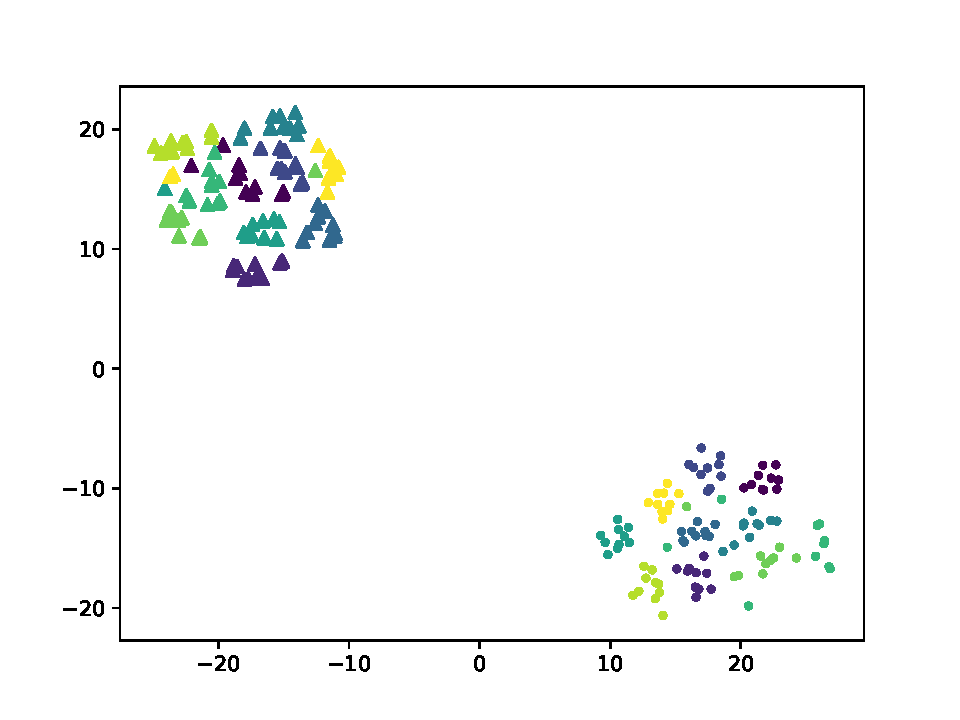
\includegraphics{tsne.pdf}
	\label{fig:tsne}
	\caption[t-SNE Plot of Universal Perturbations]{Two dimensional embedding of the universal perturbations on CIFAR-10 calculated using t-SNE \citep{tsne}. The upper right cluster represents perturbations computed on a ConvNet, whereas the cluster in the lower left represents those calculated on a CapsNet. Perturbations with the same color were created using the same subset of test data.}
\end{figure}




\subsubsection{SVD}
6
\citet{universal} considered singular values of the matrix containing normalized adversarial examples to determine, if adversarial examples lie in a low dimensional subspace. \\
For this purpose, let us denote with $\delta(x)$ the minimal adversarial perturbation for the input $x \in [0,1]^n$,
and $ N = \begin{bmatrix}
\frac{\delta(x_1)} {\norm{\delta(x_1)}},  ...,  \frac{\delta(x_k)} {\norm{\delta(x_k)}} 
\end{bmatrix}
\in \mathrm{R}^{n \times k}
$ for some $x_1, ..., x_k$ in the test set. \\
$\delta(x)$ is orthogonal to the decision boundary, assuming it is reasonably smooth, therefore the singular values of N give us information about the decision boundary. For example, for an binary linear classifier, N would have a rank of one, i.e. only one non-zero singular value.

In this regard we find little difference between CapsNets and ConvNets.

\begin{figure}
	\caption{Singular Values of Matrix Containing Normal Vectors To the Decision Boundary}
	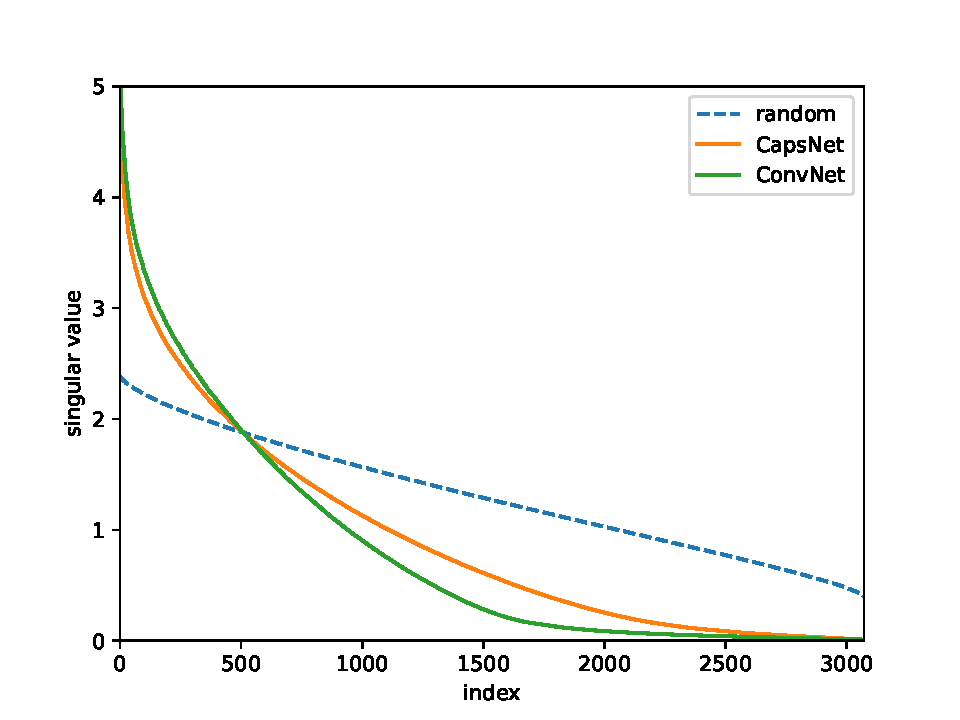
\includegraphics{svd_cifar10.pdf}
	\label{fig:svd}
\end{figure}
